%%
%% This is file `mcmthesis-demo.tex',
%% generated with the docstrip utility.
%%
%% The original source files were:
%%
%% mcmthesis.dtx  (with options: `demo')
%% !Mode:: "TeX:UTF-8"
%% -----------------------------------
%% This is a generated file.
%% 
%% Copyright (C) 2010 -- 2015 by latexstudio
%%       2014 -- 2019 by Liam Huang
%%       2019 -- present by latexstudio.net
%% 
%% License: The LaTeX Project Public License 1.3c
%% 
%% The Current Maintainer of this work is latexstudio.net.
%% 

\documentclass{mcmthesis}
 %\documentclass[CTeX = true]{mcmthesis}  % 当使用 CTeX 套装时请注释上一行使用该行的设置
\mcmsetup{tstyle=\color{red}\bfseries,%修改题号,队号的颜色和加粗显示,黑色可以修改为 black
        tcn = 2524908, problem = C, %修改队号,参赛题号
        sheet = true, titleinsheet = false, keywordsinsheet = true,%修改sheet显示信息
        titlepage = false, abstract = true}

  %四款字体可以选择
  %\usepackage{times}
  %\usepackage{newtxtext,newtxmath} %CTeX 无此字体,可用 txfonts 替代,请使用新版 TeXLive.
 \usepackage[utf8]{inputenc}
 \usepackage{palatino}
  %\usepackage{txfonts}
\usepackage{enumitem}
\usepackage{float}
\usepackage{graphicx}
\usepackage{tabularx}
\graphicspath{ {./figures/} }
\usepackage{indentfirst}  %首行缩进,注释掉,首行就不再缩进。
\usepackage{csquotes}
\usepackage{longtable}
\usepackage{tikz}
\usepackage[backend=biber, style=authoryear]{biblatex}
\addbibresource{refs.bib}
\usetikzlibrary{shapes.geometric, arrows}
\tikzstyle{startstop} = [rectangle, rounded corners, text centered, draw=black, fill=red!30]
\tikzstyle{process} = [rectangle, text centered, draw=black, fill=blue!30]
\tikzstyle{arrow} = [thick,->,>=stealth]
\title{MCM Problem C}
\author{\small \href{https://www.latexstudio.net/}
  {
\includegraphics{mcmthesis-logo}}}
\date{\today}
\usepackage[hang,flushmargin]{footmisc}
\usepackage{hyperref}
\hypersetup{
    colorlinks=true,
    linkcolor=black,
    urlcolor=blue,
    citecolor=gray
}
\begin{document}
\begin{abstract}
\par %Use this template to begin typing the first page (summary page) of your electronic report. This
%template uses a 12-point Times New Roman font. Submit your paper as an Adobe PDF
%electronic file (e.g. 1111111.pdf), typed in English, with a readable font of at least 12-point type. 

%Do not include the name of your school, advisor, or team members on this or any page. 

%Be sure to change the control number and problem choice above. 

%You may delete these instructions as you begin to type your report here.  

%\textbf{Follow us @COMAPMath on Twitter or COMAPCHINAOFFICIAL on Weibo for the
%most up to date contest information.}
\begin{Abstract}
In this paper, we construct several models to predict the success of the 2028 Los Angeles Olympic Games. Our dataset contains the total scores for nearly 1000 countries and regions from 1896 to 2024. We built an artificial neural network model and a multiple linear regression model to predict the results of the 2028 Olympic Games. Then, we used the entropy-weighted method to integrate these two different outcomes to gain the synthetic results. We also find the relationship between the events and the number of medals gained and compare the performance of each country in the 2024 Olympic Games and their performance in the 2028 Olympic Games to determine which country will perform better and which country will perform worse.
\end{Abstract}
\begin{keywords}
Multiple Linear Regression; Neural Network; Entropy-weighted Method
\end{keywords}
\end{abstract}
\maketitle
%% Generate the Table of Contents, if it's needed.
\tableofcontents
\newpage
%%
%% Generate the Memorandum, if it's needed.
%% \memoto{\LaTeX{}studio}
%% \memofrom{Liam Huang}
%% \memosubject{Happy \TeX{}ing!}
%% \memodate{\today}
%% \memologo{\LARGE I'm pretending to be a LOGO!}
%% \begin{memo}[Memorandum]
%%   \lipsum[1-3]
%% \end{memo}
%%
\section{Introduction}

\subsection{Background}

The Olympic Games have long served as a global stage where athletes from diverse backgrounds come together to compete at the highest level. Scheduled to take place in Los Angeles, California, the 2028 Summer Olympics mark the city’s third time hosting this prestigious event, following its successful iterations in 1932 and 1984.

As the Games approach, attention is increasingly focused on the potential medal outcomes, which reflect not only the athletes’ dedication but also the geopolitical, cultural, and economic forces shaping global sports. Nations are investing heavily in sports programs, science-backed training methods, and athlete development, with the aim of achieving their position on the medal table. At the same time, emerging powers in international sports are challenging the dominance of traditional medal-winning nations, hinting at a potential reshaping of the competitive landscape in 2028.

This paper explores these dynamics within the unique context of the Los Angeles Games, including its innovative event lineup, the past performances of each country and the composition of each national team.

\subsection{Framework of Analysis}
In this paper, we established multiple models to predict the medals earned of each country in the 2028 Olympic Games held in Los Angeles. The first model we take is the artificial neural network (ANN). The neural network program is constructed using Python and trained with the databases provided by the organizer of this competition. The databases we used included data about the names of athletes and the countries they represent, the hosting country, the medals awarded, and the hosting year from 1896 to 2024 of each country. The other model we take is multiple linear regression (MLR). In this model, we find the linear relationships between the variables in the database and the medals earned of each country. To find the synthetic results from these two outcomes of different methods, we take the entropy-weight method (EWM) to calculate the weight between the data from each method. Eventually, we will take the weighted average value to obtain the final result.  

\subsection{Comments on Data Provided}
There have been many inconsistencies we observed in the provided data, many of which were not addressed in the problem statement. Nonetheless, we have found ways to circumvent these errors to create working models regardless. First, we must address the issue of the 1906 Summer Olympics. While running tests on the multidimensional regression model we found an error in which the model handled one specific date, namely the 1906 Olympics. After closer reading, it came to out attention that the 1906 Olympics did not follow the standard 4 year gap between events. This was cumbersome because this information was only stored in the athletes data file, and not mentioned in neither the medal count file nor the host file. This deleted crucial information on which the regression model bases its predictions on. We have elected not to include those Olympics in the regression model, due to the stipulation not to use any external data (i.e. data from sources others than the ones provided). It had been included, however, in the neural network model, as there need not be for extremely precise definitions compared to the regression model; however, this might be contributing to some amount of error (formally called \textit{loss} in machine learning environments).
We have also found errors in the files themselves. There are certain characters at the end of some team names that inhibit complete data analysis on the unmodified provided files. These include, but are not limited to, the characters " " being concatenated to the end of country names in the \texttt{medal\_counts.csv} file for the 1932 and 1960 Olympics, the existence of "subteams" like Japan-1 or United States-13, or the aforementioned lack of host data for the special 1906 Summer Olympics. Although it is difficult to predict what influence these errors had on the neural network model, we found ways to circumvent these issues when working with the regression model. 

\section{Analysis of the Problem}

\subsection{The Artificial Neural Network}
The artificial neural network was coded in Python 3.12.0, with the help of standard machine learning (ML) and data analysis libraries: \href{https://pandas.pydata.org/}{\texttt{Pandas}}, \href{https://numpy.org/}{\texttt{NumPy}}, \href{https://scikit-learn.org/stable/}{\texttt{scikit-learn}} and \href{https://www.tensorflow.org/}{\texttt{TensorFlow}}. The raw code may be found in Appendix A after following the github link. The Artificial Neural Network (henceforth abbreviated as ANN) was trained on three of the four provided files: \texttt{summerOly\_atheletes.csv}, \texttt{summerOly\_hosts.csv}, \\ \texttt{summerOly\_medal\_counts.csv}. The ANN was designed with three layers, the input layer (with 32 neurons), the middle layer (with 16 neurons) and the output layer (with 1 neuron). After each training iteration, the ANN prunes (omits) random neurons and connections (20\% for this ANN) to prevent overfitting and force the ANN to learn the patterns visible in the training data. This is done to prevent the ANN from depending on any specific neuron, which is common in smaller ANN's (like the one created for this paper) or with a relatively small amount of training data (also the case in this problem). An example of a pruned neural network is shown in Figure~\ref{figure: NN}. The data followed the standard 90/10 split, whereby 90\% of the data was used to train the model, and 10\% to test the models accuracy. Rectified Linear Unit (ReLU) was chosen as the activation function for the first 2 ANN layers, due to the many benefits it provides over other functions like Sigmoid, which tend to slow the model down during backpropagation, since it confines all inputs into the range $[0, 1]$. For very large or small input values, the gradient is disproportionally closer to 0, which significantly slows down the updating of weights between neurons. Although many slightly different variations of the ReLU function exist, the ANN used the function defined as $x\mapsto \max(0, x)$.

\begin{figure} [H]
    \centering
    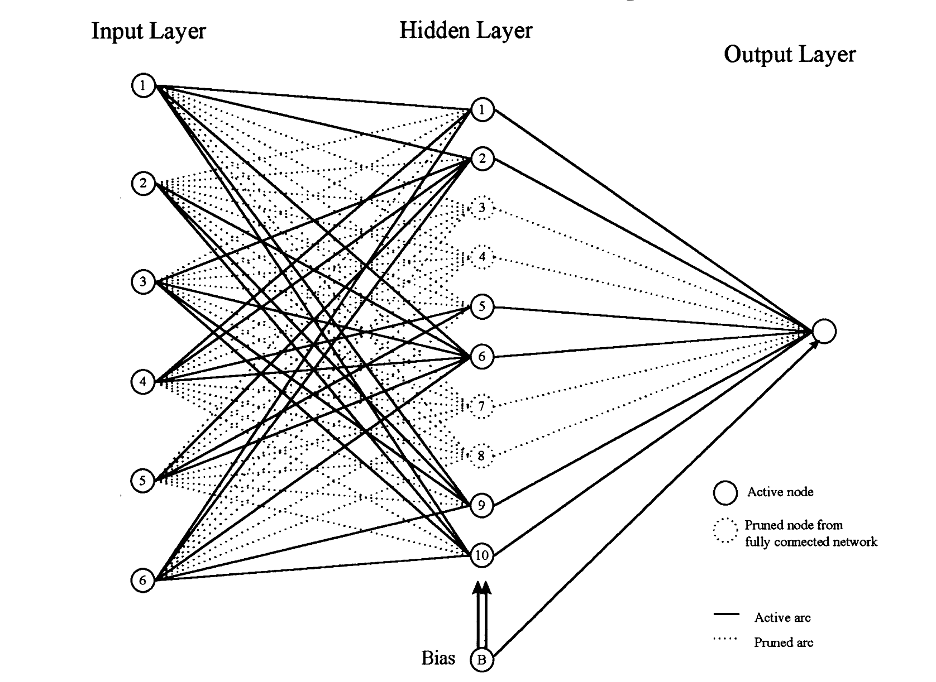
\includegraphics[width=0.95\textwidth]{prunes-nn-vis}
    \caption{Example of pruned neural network}
    \label{exampleID}
    \label{figure: NN}
\end{figure}

The final layer was standardized using the Softmax function, again as is custom in multilayer classification neural networks. Softmax standardizes the outputs to be a valid probability distribution, defined as:
\begin{equation}\label{eq:softmax}
    \text{Softmax}(z_i) = \frac{e^{z_i}}{\sum_{j=1}^{n} e^{z_j}}
\end{equation}
The ANN also used three additional functions to calculate its effectiveness. The optimizer Adam (Adaptive Moment Estimation) function was used to minimize the loss function dynamically, by changing the weights and biases of neurons and connections. It ensures the neural network converges to a good solution efficiently. It is defined mathematically below:
\begin{align}\label{eq:adam func}
    \begin{split}
    &\omega_{t+1}=\omega_t-\alpha m_t\\
    &m_t = \beta m_{t+1} + (1-\beta) \left[\frac{\partial L}{\partial \omega_t} \right]
    \end{split}
\end{align}

\begin{table}[H]
\caption{Variable Definitions for Equation~(\ref{eq:adam func})}
\centering
\begin{tabularx}{\textwidth} {
  >{\raggedright\arraybackslash}X 
  >{\raggedright\arraybackslash}X  }
 \hline
 \textbf{Variable} & \textbf{Definition} \\
 \hline\hline
  $t_0$ & Initial time, $t_0 = 0$ \\
 $m_t$ & Aggregate of gradients at $t$ ($m_{t_0}=0$) \\
 $m_{t-1}$ & Aggregate of gradients at $t_\text{previous}$ \\
 $\omega_{t}$ & Weights at $t$ \\ 
 $\omega_{t+1}$ & Weights at $t\equiv t+1$ \\ 
 $\alpha_t$ & Learning rate at $t$ \\ 
 $\partial L$ & Derivative of the loss function \\ 
 $\partial \omega_t$ & Derivative of weights at $t$ \\
 $\beta$ & Moving average parameter, const. \\
 \hline
\end{tabularx}
\end{table}

The loss function was chosen to be \textit{Binary Cross Entropy} (also known as \textit{log loss}). The neural network was punished when loss was high, which leads to the ANN learning the data. The Binary Cross Entropy function is defined as:
\begin{equation}\label{eq:binary crossentropy}
    \text{BCE} = -\frac{1}{N}\sum_{i=0}^{N}\left [y_i \log(p_i) +(1-y_i)\log(1-p_i)\right]
\end{equation}
\begin{table}[!htbp]
\caption{Variable definition for Equation~(\ref{eq:binary crossentropy})}
\centering
\vspace{5pt}
\begin{tabularx}{\textwidth} {
  >{\raggedright\arraybackslash}X 
  >{\raggedright\arraybackslash}X  }
 \hline
 \textbf{Variable} & \textbf{Definition} \\
 \hline\hline
  $N$ & Number of instances \\
  $y_i$ & True label for instance $i$ \\
 $p_i$ & Model predicted probability of instance $i$ \\ \hline
 \end{tabularx}
\end{table}

\subsubsection{Model Performance}

Full results of ANN predictions may be found in Section~\ref{sec:results-integration}. This section will be dedicated to providing the results for the ANN itself. The ANN used $n=50$ epochs for training, to ensure maximum accuracy of the model and minimize the risk of potential overfitting. The final values for key metrics are shown in the table below.

\begin{table}[H]
\caption{Key ANN metrics}
\centering
\vspace{5pt}
\begin{tabularx}{\textwidth} {
  >{\raggedright\arraybackslash}X 
  >{\raggedright\arraybackslash}X  }
\hline
 \textbf{Metric} & \textbf{Value} \\   
 \hline\hline
  Training Accuracy & $0.9976$\\ 
  Training Loss & $0.0173$\\
 Validation Accuracy & $0.9250$\\
 Validation Loss & $0.2187$\\ \hline
\end{tabularx}
\end{table}

Although it is not possible to fully understand how the neural network learned the data, the four above metrics give insight into its workings on both training and validation (testing) data. Looking at the training metrics first, it becomes clear the model handles seen data exceptionally well, with an extremely high training accuracy and very low training loss. Usually, this means the neural network is extremely well trained. In this case, however, it may point towards overfitting, since the winners of events are (somewhat) random. Having a $0.9976$ and $0.0173$ training accuracy and loss on a slightly random data set is a first indication of overfitting in the model. However, the ANN still fairs well with data it has not yet seen, as evidenced by the relatively high validation accuracy. The increase in loss value from training to validation does support the overfitting hypothesis, however it is well within accepted ranges for well trained neural networks, meaning the predictions of the ANN may be accepted as valid.

\subsection{Multiple Linear Regression}\label{sec:mlr}

Since ANNs are designed for non-linear data and trends (due to non-linear activation functions), we thought it best to also model the given data in a way that could capture any linearity in the structure of our given data or within any trends in the data. Previous work that we on using linear regression to make predictions about the Olympics made use of data that was not available in our dataset, such as socioeconomic metrics like as GDP and HDI~\parencite{reg:2009}, and details on athletes like height and weight~\parencite{reg:2024}. Since we did not have access to this kind of data in this problem, we instead tested for correlations between each country's medal counts (bronze, silver, gold, and total) and the following parameters:

\begin{description}[style=nextline,font=\normalfont]
    \item[\texttt{Athletes}] Number of athletes that competed for the country.
    \item[\texttt{Sports}] Number of sports that the country participated in.
    \item[\texttt{Events}] Number of events that the country participated in.
    \item[\texttt{Is.host}] A flag that is 1 if the country is the host, and 0 otherwise.
    \item[\texttt{Mean.Sex}] For each country's athletes in a given year, we set their sex to 0 if they were female and 1 if they were male. \texttt{Mean.Sex} gives the mean of these values. Thus, the higher this predictor, the larger the percentage of athletes was male.
    \item[\texttt{Mean.Sport.Participation}] For each year, we made a dictionary that counted the number of countries that competed in given sports. For each country in a given year, we indexed this dictionary only at the sports that this country participated in, and took the mean of the corresponding values. Intuitively, this could be thought of as the \enquote{mean popularity} of the sports that this country participated in for this year.
    \item[\texttt{Mean.Event.Participation}] Same as \texttt{Mean.Sport.Participation}, only with events.
    \item[\texttt{Bronze.Last.Olympics}] Number of Bronze medals won in the last year. 
    \item[\texttt{Silver.Last.Olympics}] Number of Silver medals won in the last year. 
    \item[\texttt{Gold.Last.Olympics}] Number of Gold medals won in the last year. 
\end{description}

The full table containing all of these parameters for each country in each year can be found in \href{https://github.com/YanxiangShan/MCM-2524908/blob/main/code/MLR/processed_data.csv}{\texttt{processed\_data.csv}}, and the code that generated this table can be found in \href{https://github.com/YanxiangShan/MCM-2524908/blob/main/code/MLR/process_data.R}{\texttt{process\_data.R}}. As a final note with respect to the data, we found 20 outliers in the data that are \enquote{extreme} with respect to the dependent variable according to studentized deleted residuals, and none that are \enquote{extreme} with respect to any independent variables according to the hat values metric.

Using these parameters and their respective data, we constructed four multiple linear regression models, one for each medal type and another for total medals\footnote{
    All tables in section~\ref{sec:mlr} were generated by the R package \texttt{stargazer}---see~\cite{hlavac2022stargazer} for a preview.
}:

% Table created by stargazer v.5.2.3 by Marek Hlavac, Social Policy Institute. E-mail: marek.hlavac at gmail.com
% Date and time: Mon, Jan 27, 2025 - 6:37:41 PM
\begin{longtable}{@{\extracolsep{5pt}}lcccc} 
  \caption{Full MLR Model} 
  \label{} 
\\[-1.8ex]\hline 
\hline \\[-1.8ex] 
 & \multicolumn{4}{c}{\textit{Dependent variable:}} \\ 
\cline{2-5} 
\\[-1.8ex] & Bronze & Silver & Gold & Total \\ 
\\[-1.8ex] & (1) & (2) & (3) & (4)\\ 
\hline \\[-1.8ex] 
 Constant & 3.850$^{***}$ & 3.875$^{***}$ & 3.681$^{***}$ & 11.406$^{***}$ \\ 
  & p = 0.0001 & p = 0.0001 & p = 0.002 & p = 0.00002 \\ 
  & & & & \\ 
 Athletes & 0.034$^{***}$ & 0.042$^{***}$ & 0.039$^{***}$ & 0.115$^{***}$ \\ 
  & p = 0.000 & p = 0.000 & p = 0.000 & p = 0.000 \\ 
  & & & & \\ 
 Sports & $-$0.154$^{***}$ & $-$0.121$^{***}$ & $-$0.109$^{***}$ & $-$0.384$^{***}$ \\ 
  & p = 0.00002 & p = 0.001 & p = 0.008 & p = 0.0001 \\ 
  & & & & \\ 
 Events & $-$0.003 & $-$0.034$^{***}$ & $-$0.038$^{***}$ & $-$0.075$^{***}$ \\ 
  & p = 0.684 & p = 0.00002 & p = 0.00002 & p = 0.0004 \\ 
  & & & & \\ 
 Is.host & 21.610$^{***}$ & 21.297$^{***}$ & 17.014$^{***}$ & 59.920$^{***}$ \\ 
  & p = 0.000 & p = 0.000 & p = 0.000 & p = 0.000 \\ 
  & & & & \\ 
 Mean.Sex & $-$2.654$^{***}$ & $-$2.759$^{***}$ & $-$2.827$^{***}$ & $-$8.240$^{***}$ \\ 
  & p = 0.002 & p = 0.001 & p = 0.003 & p = 0.0003 \\ 
  & & & & \\ 
 Mean.Sport.Participation & $-$0.001$^{***}$ & $-$0.001$^{**}$ & $-$0.001$^{*}$ & $-$0.002$^{**}$ \\ 
  & p = 0.006 & p = 0.047 & p = 0.096 & p = 0.015 \\ 
  & & & & \\ 
 Mean.Event.Participation & $-$0.002 & $-$0.003$^{**}$ & $-$0.002 & $-$0.006$^{**}$ \\ 
  & p = 0.117 & p = 0.015 & p = 0.130 & p = 0.037 \\ 
  & & & & \\ 
 Bronze.Last.Olympics & 0.182$^{***}$ & 0.127$^{***}$ & 0.018 & 0.328$^{***}$ \\ 
  & p = 0.00001 & p = 0.002 & p = 0.693 & p = 0.003 \\ 
  & & & & \\ 
 Silver.Last.Olympics & $-$0.015 & 0.003 & $-$0.001 & $-$0.013 \\ 
  & p = 0.739 & p = 0.941 & p = 0.988 & p = 0.920 \\ 
  & & & & \\ 
 Gold.Last.Olympics & 0.277$^{***}$ & 0.365$^{***}$ & 0.627$^{***}$ & 1.270$^{***}$ \\ 
  & p = 0.000 & p = 0.000 & p = 0.000 & p = 0.000 \\ 
  & & & & \\ 
 Events:Is.host & $-$0.112$^{***}$ & $-$0.095$^{***}$ & $-$0.046$^{***}$ & $-$0.252$^{***}$ \\ 
  & p = 0.000 & p = 0.000 & p = 0.004 & p = 0.000 \\ 
  & & & & \\ 
 Is.host:Mean.Event.Participation & 0.003 & $-$0.001 & $-$0.009 & $-$0.006 \\ 
  & p = 0.599 & p = 0.862 & p = 0.246 & p = 0.718 \\ 
  & & & & \\ 
\hline \\[-1.8ex] 
Observations & 1,045 & 1,045 & 1,045 & 1,045 \\ 
R$^{2}$ & 0.756 & 0.772 & 0.776 & 0.812 \\ 
Adjusted R$^{2}$ & 0.754 & 0.769 & 0.774 & 0.810 \\ 
Akaike Inf. Crit. & 5,634.121 & 5,623.582 & 5,939.055 & 7,747.321 \\ 
Bayesian Inf. Crit. & 5,703.446 & 5,692.907 & 6,008.380 & 7,816.646 \\ 
Residual Std. Error (df = 1032) & 3.560 & 3.542 & 4.119 & 9.784 \\ 
F Statistic (df = 12; 1032) & 266.964$^{***}$ & 290.373$^{***}$ & 298.126$^{***}$ & 371.542$^{***}$ \\ 
\hline 
\hline \\[-1.8ex] 
\textit{Note:}  & \multicolumn{4}{r}{$^{*}$p$<$0.1; $^{**}$p$<$0.05; $^{***}$p$<$0.01} \\ 
\end{longtable} 

We see that nearly all of our predictors have very small p-values, meaning nearly all of them are significant, including the metrics related to sports and events. The only exception is \texttt{Silver.Last.Olympics}, which shows the opposite effect---its p-values are very large, indicating that the number of silver medals a country has is. When analyzing our correlations, we focus only the model with the total number of medals as the dependent variable to reduce redundancy, as our analyses were identical for all models. 

\subsubsection{Backwards Model Selection}

This model has a great deal of unnecessary predictors, as shown by the low p-values. We will use the backwards selection algorithm provided by the R package \texttt{MASS} to select smaller models. After backwards selection, we have the following information of our models:

% Table created by stargazer v.5.2.3 by Marek Hlavac, Social Policy Institute. E-mail: marek.hlavac at gmail.com
% Date and time: Mon, Jan 27, 2025 - 6:49:47 PM
\begin{table}[!htbp] \centering 
  \caption{} 
  \label{} 
\begin{tabular}{@{\extracolsep{5pt}}lcccc} 
\\[-1.8ex]\hline 
\hline \\[-1.8ex] 
 & \multicolumn{4}{c}{\textit{Dependent variable:}} \\ 
\cline{2-5} 
\\[-1.8ex] & Bronze & Silver & Gold & Total \\ 
\\[-1.8ex] & (1) & (2) & (3) & (4)\\ 
\hline \\[-1.8ex] 
 Athletes & 0.034$^{***}$ & 0.042$^{***}$ & 0.039$^{***}$ & 0.114$^{***}$ \\ 
  & p = 0.000 & p = 0.000 & p = 0.000 & p = 0.000 \\ 
  & & & & \\ 
 Sports & $-$0.152$^{***}$ & $-$0.122$^{***}$ & $-$0.115$^{***}$ & $-$0.388$^{***}$ \\ 
  & p = 0.00002 & p = 0.001 & p = 0.005 & p = 0.0001 \\ 
  & & & & \\ 
 Events & $-$0.004 & $-$0.034$^{***}$ & $-$0.036$^{***}$ & $-$0.074$^{***}$ \\ 
  & p = 0.646 & p = 0.00002 & p = 0.00003 & p = 0.0005 \\ 
  & & & & \\ 
 Is.host & 21.661$^{***}$ & 21.278$^{***}$ & 16.811$^{***}$ & 59.787$^{***}$ \\ 
  & p = 0.000 & p = 0.000 & p = 0.00000 & p = 0.000 \\ 
  & & & & \\ 
 Mean.Sex & $-$2.630$^{***}$ & $-$2.766$^{***}$ & $-$2.866$^{***}$ & $-$8.264$^{***}$ \\ 
  & p = 0.002 & p = 0.001 & p = 0.003 & p = 0.0003 \\ 
  & & & & \\ 
 Mean.Sport.Participation & $-$0.001$^{***}$ & $-$0.001$^{**}$ & $-$0.001$^{*}$ & $-$0.002$^{**}$ \\ 
  & p = 0.006 & p = 0.045 & p = 0.082 & p = 0.014 \\ 
  & & & & \\ 
 Mean.Event.Participation & $-$0.002 & $-$0.003$^{**}$ & $-$0.002 & $-$0.006$^{**}$ \\ 
  & p = 0.126 & p = 0.014 & p = 0.111 & p = 0.034 \\ 
  & & & & \\ 
 Bronze.Last.Olympics & 0.177$^{***}$ & 0.128$^{***}$ &  & 0.321$^{***}$ \\ 
  & p = 0.00000 & p = 0.0003 &  & p = 0.002 \\ 
  & & & & \\ 
 Gold.Last.Olympics & 0.270$^{***}$ & 0.367$^{***}$ & 0.638$^{***}$ & 1.265$^{***}$ \\ 
  & p = 0.000 & p = 0.000 & p = 0.000 & p = 0.000 \\ 
  & & & & \\ 
 Events:Is.host & $-$0.110$^{***}$ & $-$0.095$^{***}$ & $-$0.050$^{***}$ & $-$0.255$^{***}$ \\ 
  & p = 0.000 & p = 0.000 & p = 0.002 & p = 0.000 \\ 
  & & & & \\ 
 Constant & 3.803$^{***}$ & 3.889$^{***}$ & 3.770$^{***}$ & 11.458$^{***}$ \\ 
  & p = 0.0001 & p = 0.0001 & p = 0.001 & p = 0.00002 \\ 
  & & & & \\ 
\hline \\[-1.8ex] 
Observations & 1,045 & 1,045 & 1,045 & 1,045 \\ 
R$^{2}$ & 0.756 & 0.771 & 0.776 & 0.812 \\ 
Adjusted R$^{2}$ & 0.754 & 0.769 & 0.774 & 0.810 \\ 
Akaike Inf. Crit. & 5,630.521 & 5,619.619 & 5,934.577 & 7,743.463 \\ 
Bayesian Inf. Crit. & 5,689.943 & 5,679.041 & 5,989.046 & 7,802.884 \\ 
% Residual Std. Error & 3.557 (df = 1034) & 3.538 (df = 1034) & 4.116 (df = 1035) & 9.775 (df = 1034) \\ 
% F Statistic & 320.815$^{***}$ (df = 10; 1034) & 349.106$^{***}$ (df = 10; 1034) & 397.909$^{***}$ (df = 9; 1035) & 446.641$^{***}$ (df = 10; 1034) \\ 
\hline 
\hline \\[-1.8ex] 
\textit{Note:}  & \multicolumn{4}{r}{$^{*}$p$<$0.1; $^{**}$p$<$0.05; $^{***}$p$<$0.01} \\ 
\end{tabular} 
\end{table} 

We see that the predictors \texttt{Silver.Last.Olympics} and \\ \texttt{Is.host:Mean.Event.Participation}, the interaction term, were dropped from every model, and \texttt{Bronze.Last.Olympics} was dropped specifically from the Gold model. We will use these models in all predictions and in the following sections.

\subsubsection{Multicollinearity}\label{ssec:vif}

Measuring multicollinearity in each predictor is important to determine how independent their effects are on the full model. If a given predictor is multicollinear, it is common for it to have a small p-value in a MLR model, but a small p-value in a SLR model, or vice versa. We measure multicollinearity using Variance Inflation Factors (VIF). The functionality to calculate this is provided by the R package \texttt{cars}. The VIFs for each predictor from each model is given below. Note that We only show the VIF values for the model of total medals because the respective values for the predictors in the other models are nearly identical. See \href{https://github.com/YanxiangShan/MCM-2524908/blob/main/code/MLR/analysis/vifs.csv}{\texttt{vifs.csv}} for the full table with data for all models, or \href{https://github.com/YanxiangShan/MCM-2524908/blob/main/code/MLR/analysis/vifs.csv}{\texttt{vif\_diffs.csv}} for the difference between all VIFs and the VIFs from the Total column.

% Table created by stargazer v.5.2.3 by Marek Hlavac, Social Policy Institute. E-mail: marek.hlavac at gmail.com
% Date and time: Mon, Jan 27, 2025 - 3:58:41 PM
\begin{longtable}{@{\extracolsep{5pt}} l|c} 
  \caption{VIF values for each predictor in the total model} 
  \label{tbl:vif} 
\\[-1.8ex]\hline 
\hline \\[-1.8ex] 
Predictor & VIF \\ 
\hline
Athletes & $12.654$ \\ 
Sports & $6.685$ \\ 
Events & $14.315$ \\ 
Is.host & $1.524$ \\ 
Mean.Sex & $1.798$ \\ 
Mean.Sport.Participation & $1.440$ \\ 
Mean.Event.Participation & $1.329$ \\ 
Bronze.Last.Olympics & $6.252$ \\ 
Silver.Last.Olympics & $8.385$ \\ 
Gold.Last.Olympics & $6.850$ \\ 
\hline
\end{longtable} 

We usually note that a predictor exhibits multicollinearity if its VIF value exceeds 10. Correspondingly, we see the values for \texttt{Athletes} and \texttt{Events} exceeded 10, indicating multicollinearity in these particular parameters, but none others. Testing these parameters individually gives the following results:

% Table created by stargazer v.5.2.3 by Marek Hlavac, Social Policy Institute. E-mail: marek.hlavac at gmail.com
% Date and time: Mon, Jan 27, 2025 - 2:09:47 AM
\begin{longtable}{@{\extracolsep{5pt}}lcc} 
    \caption{}
    \label{}
\\[-1.8ex]\hline 
\hline \\[-1.8ex] 
 & \multicolumn{2}{c}{\textit{Dependent variable:}} \\ 
\cline{2-3} 
\\[-1.8ex] & \multicolumn{2}{c}{Total} \\ 
\\[-1.8ex] & (1) & (2)\\ 
\hline \\[-1.8ex] 
 Sports & 1.390$^{***}$ &  \\ 
  & p = 0.000 &  \\ 
  & & \\ 
 Events &  & 0.259$^{***}$ \\ 
  &  & p = 0.000 \\ 
  & & \\ 
 Constant & $-$6.570$^{***}$ & $-$4.901$^{***}$ \\ 
  & p = 0.000 & p = 0.000 \\ 
  & & \\ 
\hline \\[-1.8ex] 
Observations & 1,419 & 1,419 \\ 
R$^{2}$ & 0.270 & 0.452 \\ 
Adjusted R$^{2}$ & 0.270 & 0.452 \\ 
Residual Std. Error (df = 1417) & 18.448 & 15.983 \\ 
F Statistic (df = 1; 1417) & 525.181$^{***}$ & 1,170.515$^{***}$ \\ 
\hline 
\hline \\[-1.8ex] 
\textit{Note:}  & \multicolumn{2}{r}{$^{*}$p$<$0.1; $^{**}$p$<$0.05; $^{***}$p$<$0.01} \\ 
\end{longtable} 

Thus, we see that with respect to p-values, although these predictors exhibit multicollinearity, they are relevant to their models regardless of the presence of all other predictors. 

% This is further supported by running a backwards selection algorithm on the full model, which elects only to eliminate the \texttt{Silver.Last.Olympics} predictor according to AIC, which possesses the highest p-value of all of the parameters by far (we do not use this model when making predictions in further sections).

\subsubsection{Error Variance Constancy (Total model)}

We use a Modified Levene Test (see Appendix~\ref{ap:mlt} for details) on each predictor in the Total model to detect non-constant error variance. This gave the following results:

% Table created by stargazer v.5.2.3 by Marek Hlavac, Social Policy Institute. E-mail: marek.hlavac at gmail.com
% Date and time: Mon, Jan 27, 2025 - 4:28:37 PM
\begin{table}[!htbp] \centering 
  \caption{} 
  \label{tbl:mlt} 
\begin{tabular}{@{\extracolsep{5pt}} cc} 
\\[-1.8ex]\hline 
\hline \\[-1.8ex]
Predictor & p-value \\ 
\hline
Athletes & $0.149$ \\ 
Sports & $0.058$ \\ 
Events & $0.046$ \\ 
Is.host & $0.803$ \\ 
Mean.Sex & $0.054$ \\ 
Mean.Sport.Participation & $0.079$ \\ 
Mean.Event.Participation & $0.039$ \\ 
Bronze.Last.Olympics & $0$ \\ 
Silver.Last.Olympics & $0$ \\ 
Gold.Last.Olympics & $0$ \\ 
\hline \\[-1.8ex] 
\end{tabular} 
\end{table} 

Using a level $\alpha=0.05$ for this test, we see that each predictor has constant variance except for \texttt{Events}, \texttt{Mean.Event.Participation}, \texttt{Bronze.Last.Olympics}, \\ \texttt{Silver.Last.Olympics}, and \texttt{Gold.Last.Olympics}. 

\subsubsection{Influential points}

According to DFFITS, we found 16 influential points (see \href{https://github.com/YanxiangShan/MCM-2524908/tree/main/code/MLR/analysis/DFFITS.csv}{\texttt{DFFITS.csv}}); according to Cook's Distance, we found 4 influential points (see \href{https://github.com/YanxiangShan/MCM-2524908/tree/main/code/MLR/analysis/cooks_distance.csv}{\texttt{cooks\_distance.csv}}); finally, according to DFBETAS, we found 20 influential points.

\section{Results Integration}\label{sec:results-integration}

The projected medal table for the 2028 Olympics from both models is given in the table below. Note that in the predictions, the Total represents the sum of Bronze, Silver, and Gold columns, and the columns are rounded after summing. Thus, the displayed medals do not always sum to the total.

\begin{table}[H]
\centering 
\caption{Predicted 2028 Olympics Medal Table}
\label{A}
\vspace{5pt}
\begin{tabular}{l|cccc|cccc}
\hline
\textbf{Name of Country} & 
\multicolumn{4}{c}{\textbf{Artificial Neural Network}} & 
\multicolumn{4}{c}{\textbf{Multiple Linear Regression}} \\
\cline{2-5} \cline{6-9}
& Gold & Silver & Bronze & Total & Bronze & Silver & Gold & Total \\
\hline\hline
United States & 73 & 38 & 33 & 144 & 34 & 38 & 35 & 117 \\
China         & 3 & 2 & 2 & 8   & 22 & 23 & 29 & 74 \\
France        & 29 & 10 & 21 & 42  & 23 & 22 & 21 & 66 \\
Italy         & 26 & 7 & 4 & 28  & 14 & 12 & 12 & 38 \\
Germany       & 15 & 6 & 6 & 23  & 14 & 14 & 14 & 43 \\ 
$\vdots$ & $\vdots$ & $\vdots$ & $\vdots$ & $\vdots$ & $\vdots$ & $\vdots$ & $\vdots$ & $\vdots$ \\ 
Egypt         & 1 & 0 & 1 & 2   & 2 & 1 & 1 & 5 \\
Tajikistan    & 0 & 0 & 0 & 0   & 1 & 2 & 0 & 3 \\
Qatar         & 0 & 0 & 0 & 0   & 0 & 0 & 0 & 0 \\
Botswana      & 0 & 0 & 0 & 0   & 0 & 0 & 0 & 0 \\ 
\hline
\end{tabular}
\end{table}

The prediction of the neural network was standardized relative to the number of disciplines projected to be in the 2028 Olympics. Clearly, if more events are in a given Olympic, the higher the total number of medals will be, and therefore the total number of medals won by each team will be greater. Since the events and teams for the 2028 Olympics have not yet been published, we were forced to make assumptions regarding these metrics. For the medal predictions, the values were adjusted based on the number of events we assume will happen in 2028, which we took to be the exact same as in 2024. The model does account, however, for a differing number of disciplines, and can be parsed into the function to change to predictions.

However, due to the differences of these two algorithms, many differences exist between the values obtained. To solve the problem of differences in the data obtained from different methods, we need to use particular methods to combine these outcomes to get the results. To do this, we adapt the entropy-weighted method to calculate the synthetic result.

\subsection{Entropy Weight Method Model}
The entropy-weighted model is an evaluation model that determines the weights of various indicators based on the differences in the information contained in each indicator and combines the rankings derived from the proximity to the ideal solution. The specific operational flow chart is as follows:
\begin{figure}[H]
\centering
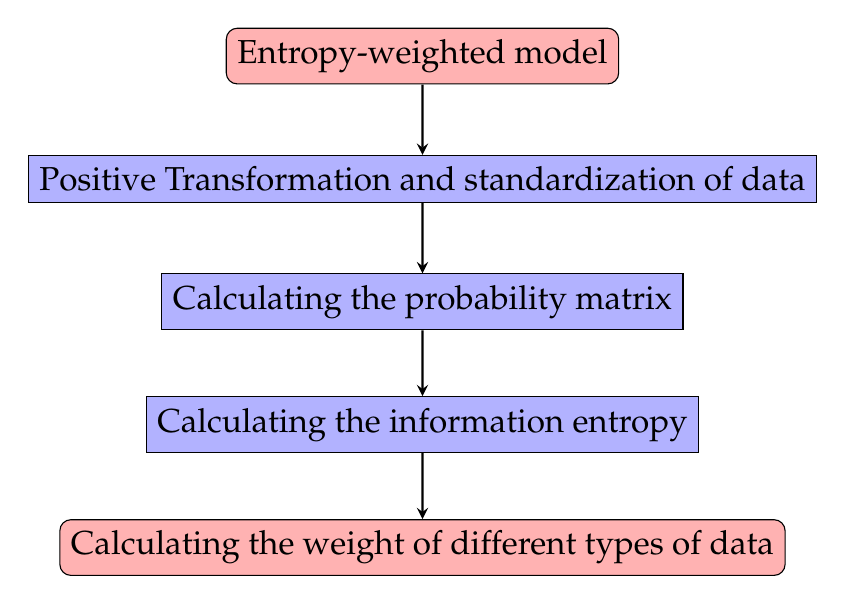
\begin{tikzpicture}[node distance=1.3cm, scale=1.2, transform shape] % 缩放到合适大小
% 定义节点
\node (start) [startstop] {Entropy-weighted model};
\node (step1) [process, below of=start] {Positive Transformation and standardization of data};
\node (step2) [process, below of=step1] {Calculating the probability matrix};
\node (step3) [process, below of=step2] {Calculating the information entropy };
\node (stop) [startstop, below of=step3] {Calculating the weight of different types of data};

% 添加箭头
\draw [arrow] (start) -- (step1);
\draw [arrow] (step1) -- (step2);
\draw [arrow] (step2) -- (step3);
\draw [arrow] (step3) -- (stop);
\end{tikzpicture}
\caption{Flowchart of The Process of EWM}
\label{fig:flowchart}
\end{figure}
In most previous competitions, most countries did not win any medals, and only very few countries gained the most, which looks like a Gamma distribution, as the figure shown below:\\
\begin{figure}[H]
  \centering
  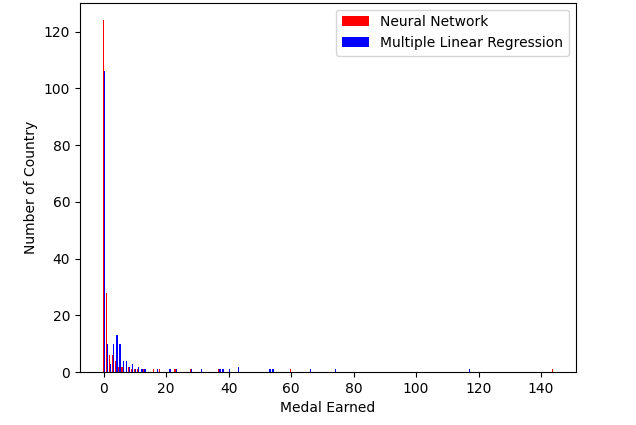
\includegraphics[width=0.95\textwidth]{myplot} % 直接写图片名字,不需要后缀
  \caption{Distributions of Total Medals Earned from both methods}
  \label{exampleId}
\end{figure}
Thus, the criteria to determine which result is more likely to be correct is to see which results about the total medals gained by each country match the Gamma distribution.\\
\begin{equation}\label{eq:1}
f(x;k,\theta) =\frac{1}{\Gamma(k) \theta^k}x^{k-1}e^{-\frac{x}{\theta}}.
\end{equation}
In this case, we are going to do the positive transformation by using the formula below:
\begin{equation}\label{K}
x_i = \frac{f(x_i) - \min(f(x))}{\max(f(x)) - \min(f(x))}
\end{equation}
The $x_i$ in(\ref{K}) is the number of total medals a particular country gains under a specific method. The data after the positive transformation is in the table below:
\begin{table}[H]
\centering 
\label{A}
\caption{Data about total medals earned after positive transformation}
\vspace{5pt}
\begin{tabular}{lcc}
\hline
\textbf{Name of the Country} & \textbf{Artificial Neural Network} & \textbf{Multiple Linear Regression} \\
\hline\hline
United States & 0 & 0\\
China & $4.06\times 10^{-1}$  & $4.18\times 10^{-13}$\\
France & $4.64\times 10^{-7}$ & $2.23\times 10^{-10}$\\
Italy & $3.17\times 10^{-4}$ & $7.82\times 10^{-6}$\\
German & $3.02\times 10^{-3}$ & $2.89\times 10^{-7}$\\
$\vdots$ & $\vdots$ & $\vdots$ \\ 
Egypt & $9.99\times 10^{-1}$ & $5.57\times 10^{-1}$\\
Kajikkistan & $8.24\times 10{-1}$ & $9.99\times 10^{-1}$\\
Qatar & $8.24\times 10{-1}$ & $8.24\times 10{-1}$\\
Botswana & $8.24\times 10{-1}$ & $8.24\times 10{-1}$\\
\hline
\end{tabular}
\end{table}
After the positive transformation, we need to normalize the data by using the formula below:\\
\begin{equation}\label{V}
\hat{x}_i=\frac{x_i}{\sqrt{x_{1}^{2}+x_{2}^{2}+\cdots+x_{n}^{2}}}
\end{equation}
In the formula~\eqref{V}, $n$ is the number of the country. Since we obtain the total medals earned by using two different method, we can use a two-dimension matrix to contain these value:\\
\begin{equation}\label{eq:3}
\tilde{x}=
\begin{bmatrix}
	x_{11}&		x_{12}\\
	x_{21}&		x_{22}\\
	\vdots&		\vdots\\
	x_{(n-1)1}&		x_{(n-1)2}\\
	x_{n1}&		x_{n2}\\
\end{bmatrix}
\end{equation}
The first column represents the total medals earned as a prediction from the artificial neural network, and the second column represents the total medals earned from the prediction of multiple linear regression.
Now, our goal changes to find the matrix:
\begin{equation}\label{eq:3}
\tilde{z}=
\begin{bmatrix}
	z_{11}&		z_{12}\\
	z_{21}&		z_{22}\\
	\vdots&		\vdots\\
	z_{\left( n-1 \right) 1}&		z_{\left( n-1 \right) 2}\\
	z_{n1}&		z_{n2}\\
\end{bmatrix}
\end{equation}
where
\begin{equation}\label{eq:1}
z_{ij}=\frac{x_{ij}}{\sqrt{x_{1j}^{2}+x_{2j}^{2}+\cdots+x_{nj}^{2}}}
\end{equation}
After gaining the normalized data of the total medals earned, we calculating the Weight matrix:
\begin{equation}\label{eq:3}
\tilde{p}= 
\begin{bmatrix}
	p_{11}&		p_{12}\\
	p_{21}&		p_{22}\\
	\vdots&		\vdots\\
	p_{(n-1) 1}&		p_{\left( n-1 \right) 2}\\
	p_{n1}&		p_{n2}\\
\end{bmatrix}
\end{equation}
where
\begin{equation}\label{eq:1}
\tilde{p}_{ij}=\frac{z_{ij}}{\sum_{i=1}^n z_{ij}}
\end{equation}
And then, we calculate the information entropy, $e_j$ of each method (ANN and MLR):
\begin{equation}\label{eq:1}
e_j=-\frac{1}{\ln n}\sum_{i=1}^n p_{ij}\ln (p_{ij}) \quad \left( j=1,2 \right)  
\end{equation}
Then, we calculate the information utility value of each type of method (ANN and MLR):
\begin{equation}\label{eq:1}
d_j=1-e_j.  
\end{equation}
Finally, we get the weight of each method by normalizing the utility values:
\begin{equation}\label{eq:1}
w_j=\frac{d_j}{d_1+d_2} \quad (j=1,2)
\end{equation}
The entropy-weighted method was coded in Python 3.12.6 with data analysis libraries NumPy, SciPy, and Pandas. The weights of each method are shown in the table below.
\begin{table}[H]
\centering 
\label{B}
\caption{Weight of Each Method}
\vspace{5pt}
\begin{tabularx}{\textwidth} {
  >{\raggedright\arraybackslash}X 
  >{\raggedright\arraybackslash}X  }
\hline
\textbf{Artificial Neural Network} & \textbf{Multiple Linear Regression} \\
\hline\hline
0.52277079 & 0.47722921\\
\hline
\end{tabularx}
\end{table}
Based on the composite weights, we calculate the weighted average of the medaas earned obtained by different methods for the same country:
\begin{equation}\label{eq:1}
\text{Medals earned} = w_\text{ANN}R_\text{ANN} + w_\text{MLR}R_\text{MLR}.
\end{equation}
$R_\text{ANN}$ is the total medals earned by a certain country calculated by the artificial neural network, and $R_\text{MLR}$ is the total medals earned by the same country calculated by the multiple linear regression. We use this to derive the final medals earned for each country as show in the next section.

\section{Projections}

\begin{table}[H]
\centering 
\label{c}
\caption{Projected Medals to be Earned for Each Country in the 2028 Olympics}
\vspace{5pt}
\begin{tabular}{lcccc}
\hline
\textbf{Country} & \textbf{Bronze} & \textbf{Silver} & \textbf{Gold} & \textbf{Total}\\
\hline\hline
United States & 33 & 38 & 60 & 131 \\
China         & 13 & 12 & 15 & 40 \\
France        & 22 & 7 & 24 & 53 \\
Italy         & 5 & 9 & 19 & 33 \\
German        & 9 & 10 & 14 & 33 \\
$\vdots$ & $\vdots$ & $\vdots$ & $\vdots$ & $\vdots$ \\
Egypt         & 1 & 1 & 1 & 3 \\
Tajikistan    & 0 & 1 & 0 & 1 \\
Qatar         & 0 & 0 & 0 & 0 \\
Botswana      & 0 & 0 & 0 & 0 \\
\hline
\end{tabular}
\end{table}

\subsection{Countries that are Projected to Improve}
To determine which country needs to work hard to improve, we established a metric, performance score, to measure a country's performance in the Olympics. We assigned unique performance scores to gold, silver, and bronze medals. The performance score for a gold medal is 5 points, for the silver medal is 3 points, and for the bronze medal is 2 points. We find each country's total score by adding the score from these three kinds of medals together to see the final performance score of each country in this Olympic Games.
We take the data in the medal table of each country in 2024 to calculate their performance score in the 2024 Olympic competition. Meanwhile, we repeat this calculation again based on the predicted data about each country's number of medals gained to get their performance score in the 2028 Olympic Games. 

A decrease in a country's performance score indicates that the country needs to put in effort to improve its current sports situation. Conversely, an increase in the performance score suggests that the country's current sports condition will likely lead to better results in the next Olympic Games.

According to the comparison of performance score, the following countries are projected to improve:

\begin{longtable}{@{\extracolsep{5pt}} ccccccc} 
  \caption{Countries that are Projected to Improve} 
  \label{} 
\\[-1.8ex]\hline 
\hline \\[-1.8ex] 
Rank & Country & Bronze & Silver & Gold & Score & Total \\ 
\hline \\[-1.8ex] 
1 & France & $23$ & $22$ & $21$ & $66$ & $217$ \\ 
2 & Australia & $18$ & $17$ & $19$ & $54$ & $182$ \\ 
3 & Japan & $17$ & $17$ & $19$ & $53$ & $180$ \\ 
4 & Germany & $14$ & $14$ & $14$ & $43$ & $140$ \\ 
5 & Ireland & $14$ & $14$ & $12$ & $40$ & $130$ \\ 
6 & Netherlands & $12$ & $12$ & $13$ & $37$ & $125$ \\ 
7 & Spain & $11$ & $11$ & $10$ & $31$ & $105$ \\ 
8 & Canada & $10$ & $9$ & $9$ & $28$ & $92$ \\ 
9 & Poland & $5$ & $4$ & $3$ & $12$ & $37$ \\ 
10 & Belgium & $4$ & $4$ & $3$ & $11$ & $35$ \\ 
11 & Denmark & $4$ & $3$ & $3$ & $9$ & $32$ \\ 
12 & Jamaica & $3$ & $3$ & $2$ & $8$ & $25$ \\ 
13 & Serbia & $2$ & $2$ & $3$ & $7$ & $25$ \\ 
14 & Kosovo & $2$ & $2$ & $2$ & $7$ & $20$ \\ 
15 & India & $3$ & $2$ & $1$ & $7$ & $17$ \\ 
16 & Chinese Taipei & $3$ & $2$ & $2$ & $7$ & $22$ \\ 
17 & North Korea & $3$ & $2$ & $2$ & $6$ & $22$ \\ 
18 & Ethiopia & $2$ & $2$ & $2$ & $6$ & $20$ \\ 
19 & Hong Kong & $2$ & $2$ & $2$ & $5$ & $20$ \\ 
20 & Bahrain & $1$ & $2$ & $2$ & $5$ & $18$ \\ 
21 & Pakistan & $2$ & $2$ & $2$ & $5$ & $20$ \\ 
22 & Ivory Coast & $2$ & $2$ & $2$ & $5$ & $20$ \\ 
23 & Indonesia & $2$ & $2$ & $2$ & $5$ & $20$ \\ 
24 & Egypt & $2$ & $1$ & $1$ & $5$ & $12$ \\ 
25 & Philippines & $2$ & $1$ & $2$ & $5$ & $17$ \\ 
26 & Kyrgyzstan & $2$ & $2$ & $1$ & $4$ & $15$ \\ 
27 & Malaysia & $2$ & $1$ & $1$ & $4$ & $12$ \\ 
28 & Slovenia & $2$ & $1$ & $2$ & $4$ & $17$ \\ 
29 & Albania & $1$ & $1$ & $1$ & $4$ & $10$ \\ 
30 & Uganda & $1$ & $1$ & $1$ & $4$ & $10$ \\ 
31 & Singapore & $1$ & $1$ & $1$ & $4$ & $10$ \\ 
32 & Dominica & $1$ & $1$ & $1$ & $3$ & $10$ \\ 
33 & Cabo Verde & $1$ & $1$ & $1$ & $3$ & $10$ \\ 
34 & Moldova & $2$ & $1$ & $1$ & $3$ & $12$ \\ 
35 & Guatemala & $1$ & $1$ & $1$ & $3$ & $10$ \\ 
36 & Panama & $1$ & $1$ & $1$ & $3$ & $10$ \\ 
37 & Mongolia & $1$ & $1$ & $1$ & $3$ & $10$ \\ 
38 & Saint Lucia & $1$ & $1$ & $1$ & $3$ & $10$ \\ 
39 & Peru & $1$ & $1$ & $1$ & $2$ & $10$ \\ 
40 & Slovakia & $1$ & $1$ & $0$ & $1$ & $5$ \\ 
\hline \\[-1.8ex] 
\end{longtable} 

\subsection{New Medalists}

There were no new medalists.

\section{Model Insights}

\subsection{Relationship between Events and Medals}

In Section~\ref{sec:mlr}, we found that the number of events a country participated in and the mean \enquote{popularity} of the events they chose to participate in (\texttt{Mean.Event.Participation}) were both relevant to all of the models of medal counts.

\subsection{``Great Coach`` Effect}

\section{Conclusions}
In this model, we construct two models to predict the total score of each country. After weighing the results of these two models, we obtain an integrated result, as shown in the table.10, the United States will win the most medals, 131. then, the following countries, France, China, Italy, and Germany, will win 53, 40, 33, and 33 medals. If we count the number of gold medals gained by each country, then the result will change to the United States winning the most gold medals, 60, and then the following countries, France, China, Italy, and Germany, will win 15, 24, 19,14.

\section{Evaluation of the Model}
Certain features of the models used in this paper work better for different questions one may have regarding the 2028 Olympics medal distribution. In truth, a combination of the ANN and MLR is useful for a more rounded overall model. While certain predictions are consistent across both models, there are crucial differences which make one better than the other in certain aspects. For example, the ANN model predicts that no new countries will win a medal in the 2028 Olympics, and it is quite easy to understand why. The model has learned that over the span of 128 years and 32 Summer Olympic Events, a particular country has not won once. On the basis of that knowledge, there is no reason why it should suggest that suddenly a country may win a medal. In this case, the linear regression model reigns supreme, as it operates on an entirely different basis, as does not fall short to the situation described above. Conversely, finding relationships of specific variables, rather than entire datasets, the MLR model is able to more accurately predict whether a country will win its first medal based on its attributes. Another consequence of the ANN learning entire data sets is a possible erroneous prediction of certain team medals. For instance, China has taken part in merely 11 Olympics, as opposed to the United States which took part in almost 30. This results in the ANN assigning China 0 medals for all Olympics it had not participated in, reinforcing a notion that China's recent successes a merely a fluke, not replicable in future events. Again, in such situations the MLR has an advantage over the ANN. The ANN model works better for conclusions requiring a view on the whole set of data, such as the influence of \textit{Host Advantage}. The MLR tries to account for this metric, but finds very little correlation, since it bases its predictions on only 1 Summer Olympic prior. This may explain the reason for a bigger discrepancy for the number of medals won by the United States than for any other country - perhaps the ANN found support for Host Advantage playing a role, and predicts the United States, as a host of the 2028 Los Angeles Olympics, will earn more medals. Many such differences exist between the two models, which is why we elected to construct both in harmony with each other. Their collective predictions should be a much more trust-worthy metric, as compared to both models in solitude.
\section{Strengths and weaknesses}


\subsection{Strengths}
\begin{itemize}
\item{We weigh multiple approaches to get the final result about how many medals each country will gain. Thus, the results will be more accurate than those from a single method.}
\end{itemize}

\subsection{Weaknesses}

\begin{itemize}
\item {Gamma distribution might not be able to exactly describe the distribution of the medals earned of each country}
\item {The ANN model takes into account all historical data, and sometimes predicts countries like the Soviet Union, Yugoslavia or Czechoslovakia as a possible winner. While the model ranks these countries very low, it ranks them nonetheless, meaning it may in theory predict that a non-existent country will win a medal, which is impossible.}

\end{itemize}

\printbibliography

\begin{appendices}

\section{Modified Levene Test (Brown-Forsythe)}\label{ap:mlt}

This test is performed to identify non-constant error variances. First, the linear regression model is fit, then residuals $e_i$ are calculated. Then, we split sample into $g$ groups, typically $g = 2$. Set group 1 to the residuals of the $n_1$ lowest values of the predictor $X$, set group 2 to the residuals of the $n_2$ highest values of the predictor $X$. We then set up the test as follows:
\[
	H_0 : \text{variance is constant}, \quad H_a : \text{variance is not constant}.
\]
Calculate $d_{i1} = |e_{i1} - \tilde{e}_{1}|$ for group 1 and $d_{i2} = |e_{i2} - \tilde{e}_{2}|$ for group 2, etc., where $e_{ij}$ is the $i$th residual of the $j$th group and $\tilde{e}_j$ is the median residual of the $j$th group. Finally, conduct a level-$\alpha$ two sample $t$-test with $d_{ij}$ using the test statistic
\[
t^* = \frac{d_{i1} - d_{i2}}{s\sqrt{\frac{1}{n_1} + \frac{1}{n_2}}},
\]
where
\[
s^2 = \frac{\sum (d_{i1} - \bar{d_1})^2 + \sum (d_{i2} - \bar{d_2})^2}{n-2}
\]
is the pooled variance. We reject $H_0$ if $|t^*| > t\left( 1-\frac{\alpha}{2} ; n - 2 \right)$, where $t\left( 1-\frac{\alpha}{2} ; n - 2 \right)$ is the $1-\frac{\alpha}{2}$ quantile of the student's t-distribution.

\end{appendices}

\AImatter

\begin{ReportAiUse}{9}

\end{ReportAiUse}

\end{document}
%% 
%% This work consists of these files mcmthesis.dtx,
%%                                   figures/ and
%%                                   code/,
%% and the derived files             mcmthesis.cls,
%%                                   mcmthesis-demo.tex,
%%                                   README,
%%                                   LICENSE,
%%                                   mcmthesis.pdf and
%%                                   mcmthesis-demo.pdf.
%%
%% End of file `mcmthesis-demo.tex'.
